% fdps_sc15.tex
% paper about FDPS for SC 15
% Author: A. Tanikawa
% 1 March 2015

\documentclass{acm_proc_article-sp}
%%%%%%%%%%%%%%%%%%%%%%%%%%%%%%%%%%%%%%%%%%%%%%%%%%%%%%%%%%%%%%%%
\usepackage{listings}
\usepackage{color}
\newcommand{\myvec}[1]{\vec{#1}}
\newcommand{\redtext}[1]{\textcolor{red}{#1}}
\newcommand{\araa}{Annual Review of Astronomy and Astrophysics}
\newcommand{\icarus}{Icarus}
\newcommand{\mnras}{Monthly Notices of the Royal Astronomical Society}
\newcommand{\apj}{Astrophysical Journal}
\newcommand{\pasa}{Publications of the Astronomical Society of Australia}
\newcommand{\pasj}{Publications of the Astronomical Society of Japan}
\newcommand{\aap}{Astronomy and Astrophysics}
%%%%%%%%%%%%%%%%%%%%%%%%%%%%%%%%%%%%%%%%%%%%%%%%%%%%%%%%%%%%%%%%

\begin{document}

\title{FDPS: A Novel Framework for Developing High-Performance
  Particle Simulation Codes for Distributed-Memory Systems}

%\subtitle{}

\numberofauthors{5}

\author{
  \alignauthor
  Masaki Iwasawa \\
  \affaddr{RIKEN Advanced Institute for Computational Science} \\
  \affaddr{7--1--26, Minatojima-minami-machi, Chuo-ku, Kobe, Hyogo, Japan} \\
  \email{masaki.iwasawa@riken.jp}
  %
  \alignauthor
  Ataru Tanikawa \\
  \affaddr{RIKEN Advanced Institute for Computational Science} \\
  \affaddr{7--1--26, Minatojima-minami-machi, Chuo-ku, Kobe, Hyogo, Japan} \\
  \email{ataru.tanikawa@riken.jp}
  %
  \alignauthor
  Natsuki Hosono \\
  \affaddr{RIKEN Advanced Institute for Computational Science} \\
  \affaddr{7--1--26, Minatojima-minami-machi, Chuo-ku, Kobe, Hyogo, Japan} \\
  \email{natsuki.hosono@riken.jp}
  \and
  %
  \alignauthor
  Keigo Nitadori \\
  \affaddr{RIKEN Advanced Institute for Computational Science} \\
  \affaddr{7--1--26, Minatojima-minami-machi, Chuo-ku, Kobe, Hyogo, Japan} \\
  \email{keigo@riken.jp}
  %
  \alignauthor
  Takayuki Muranushi \\
  \affaddr{RIKEN Advanced Institute for Computational Science} \\
  \affaddr{7--1--26, Minatojima-minami-machi, Chuo-ku, Kobe, Hyogo, Japan} \\
  \email{takayuki.muranushi@riken.jp}
  %
  \alignauthor
  Junichiro Makino \\
  \affaddr{RIKEN Advanced Institute for Computational Science} \\
  \affaddr{7--1--26, Minatojima-minami-machi, Chuo-ku, Kobe, Hyogo, Japan} \\
  \email{jmakino@riken.jp}
}

\toappear{Permission to make digital or hard copies of part or all of
  this work for personal or classroom use is granted without fee
  provided that copies are not made or distributed for profit or
  commercial advantage and that copies bear this notice and the full
  citation on the first page. Copyrights for third-party components of
  this work must be honored. For all other uses, contact the
  Owner/Author. \\ Copyright is held by the
  owner/author(s). \\ WOLFHPC2015, November 15-20 2015, Austin, TX,
  USA \\ ACM 978-1-4503-4016-8/15/11. \\
  http://dx.doi.org/10.1145/2830018.2830019}

\maketitle

\begin{abstract}

  We have developed FDPS (Framework for Developing Particle
  Simulator), which enables researchers and programmers to develop
  high-performance particle simulation codes easily.  The basic idea
  of FDPS is to separate the program code for complex parallelization
  including domain decomposition, redistribution of particles, and
  exchange of particle information for interaction calculation between
  nodes, from actual interaction calculation and orbital
  integration. FDPS provides the former part and the users write the
  latter. Thus, a user can implement, for example, a high-performance
  $N$-body code, only in 120 lines. In this paper, we present the
  structure and implementation of FDPS, and describe its performance
  on two sample applications: gravitational $N$-body simulation and
  Smoothed Particle Hydrodynamics simulation. Both codes show very
  good parallel efficiency and scalability on the K computer. FDPS
  lets the researchers concentrate on the implementation of physics
  and mathematical schemes, without wasting their time on the
  development and performance tuning of their codes.

\end{abstract}

\category{D.1.3}{Software}{PROGRAMMING TECHNIQUES}[Concurrent
  Programming]
%%
\category{I.6.7}{Computing Methodologies}{SIMULATION AND
  MODELING}[Simulation Support Systems]
%%
\category{J.2}{Computer Applications}{PHYSICAL SCIENCES AND
  ENGINEERING}[Astronomy]
%%
\category{J.2}{Computer Applications}{PHYSICAL SCIENCES AND
  ENGINEERING}[Earth and atmospheric sciences]
%%
\terms{Algorithm, Performance}
%%
\keywords{Framework for implementing parallel codes, high-performance
  computing, particle simulation}

\section{Introduction}

Particle-based simulations have been widely used in the field of
computational science, and they are becoming more and more
popular. In particle-based simulations, a system under study is
regarded as a collection of mutually-interacting particles, or
a particle system,  and its
evolution is described by the evolution (in many cases, motion) of
individual particles. Examples of particle-based simulations include
gravitational $N$-body simulation, molecular dynamics simulation,
granular dynamics simulation, and element-free simulation of fluid
dynamics or structural analysis. In the case of molecular dynamics and
gravitational $N$-body simulations, the physical system under study is
a collection of particles, and the particle-based method is a natural
way to simulate the system. Element-free methods have advantages over
structured (or unstructured) grid-based method, depending on the
nature of the system and computer system to be used. 

In order to improve the resolution and accuracy of particle-based
simulations, it is necessary to utilize present-day HPC systems.
However, to develop a calculation code for particle systems
which can achieve high efficiency on present-day HPC systems is
difficult and time-consuming. There are several reasons for this
difficulty. In order to achieve high efficiency, we need to decompose
the computational domain, assign subdomains to computing nodes, and
redistribute particles according to their positions. This
decomposition should be dynamically changed to guarantee the good load
balance. This division of the computational domain means that
computing nodes need to exchange the information of particles to
evaluate the interactions on their particles. To achieve high
efficiency, the amount of the exchanged data must be minimized, and
interaction calculation should also be efficient, making good use of
cache memory and SIMD execution units. It is also important to make
use of GPGPUs or other types of accelerators, if available.

Domain decomposition and load balance have been discussed in a number
of works \cite{1994JCoPh.111..136S, 1996NewA....1..133D,
confscWarrenSBGSW97, 2004PASJ...56..521M, ishiyama:greem,
ishiyama:gordonbell}.  The efficient use of SIMD units is discussed
in \cite{2006NewA...12..169N,2012NewA...17...82T,2013NewA...19...74T},
and GPGPUs in \cite{hamada2009novel, 2009NewA...14..630G,
Hamada:2009:THN:1654059.1654123, Hamada:2010:TAN:1884643.1884644,
2012JCoPh.231.2825B, Bedorf:2014:PGT:2683593.2683600}.

Thus, to develop a code which has all of these necessary features for
present-day HPC systems has become a big project which requires
multi-year effort of a multi-person team. It has become difficult for
researchers outside such a team to try any new experiment which
requires nontrivial modification of the code. If one wants to develop
a new numerical scheme for particle-based simulation or to apply it to
new problem, it is necessary to write his/her own code. However, it is
practically impossible for a single person, or even for a group of
people, to develop a new code which can run efficiently on present-day
HPC systems in a reasonable time.  This difficulty, in our opinion, has
slowed down the evolution of the entire field of computational science
for the last two decades. Here we discussed the situation of
particle-based codes. The situation of grid-based codes is similar. 

In order to overcome the difficulty described above, we developed FDPS
(Framework for Developing Particle
Simulator)\footnote{https://github.com/FDPS/FDPS}. Our goal is to
provide a software framework which enables researchers and programmers
to develop high-performance particle simulation codes quickly. The
basic idea of FDPS is to separate the above-described ``difficult''
part of the code, such as the domain decomposition and exchange of
particles, from the description of the physical problem itself. The
difficult part is implemented in FDPS as a library. A user of FDPS
needs to define the data structure of particles and the interaction
function of particles. Then FDPS receives these code, and generates an
efficient code to perform domain decomposition and parallelized
calculation of interaction. The user program first uses the functions
of FDPS to do the interaction calculation, and then updates the
physical data of particles, and repeats this loop until the end of
simulation.  Thus, the user of FDPS does not have to write complex
code for parallelization.

FDPS supports particle simulations with arbitrary pairwise
interactions. If the physical system includes many-body interactions,
a user can calculate such interactions within his/her code, letting
FDPS do the parallelization and calculation of pairwise interactions.
In FDPS, the separation of parallelization and physical problem is
done through the use of abstract data types implemented using C++
templates. Users of FDPS provide actual particle data class and
interaction function to the class template defined in FDPS. Thus,
users can develop a gravitational $N$-body code, Smoothed Particle
Hydrodynamics (SPH) code, other particles-based fluid code,
large-scale molecular dynamics code, a Discrete Element Method (DEM)
code, and many other particle-based code using FDPS, and all of them
will automatically parallelized with near-optimal load balancing. A
similar approach to provide general-purpose framework is
in \cite{1995CoPhC..87..266W}, but it was limited to long-range
interaction with $1/r$ potential.

One might think that, even though it is not impossible to develop
general-purpose framework for parallel particle-based simulations,
such a framework would be inevitably  slow. Since the goal of FDPS is
to make efficient use of present-day HPC systems, we designed FDPS so
that it can achieve the performance not worse than that of existing
large-scale parallel codes for particle simulations. We will discuss
the achieved performance later.

The structure of this paper is as follows. In section~\ref{sec:user},
we overview how FDPS users implement a simulation code on FDPS.  In
section~\ref{sec:implementation}, we describe parallel algorithm
implemented in FDPS. In section~\ref{sec:performance}, we illustrate
how FDPS actually simplifies the development of user programs, using
two sample FDPS applications, and describe their performance. Finally,
we summarize this study in section~\ref{sec:conclusion}.

% LocalWords:  HPC subdomains SIMD GPGPUs multi FDPS parallelized SPH
% LocalWords:  parallelization


\section{How FDPS works}
\label{sec:user}

In this section, we describe how FDPS works in detail.  In
section~\ref{sec:design}, we describe the design concept of FDPS. In
section~\ref{sec:samplecode}, we present an $N$-body simulation code
as an example, and describe how FDPS does the parallelization and what
a user program should do.

\subsection{Design and implementation}
\label{sec:design}

In this section, we describe the design and implementation of FDPS. We
first present the abstract view of calculation codes for particle-based
simulations on distributed-memory parallel computers, and then
describe how such abstraction is realized in FDPS.

\subsubsection{Abstract view of particle-based simulation codes}
\label{sec:view}

In a particle-based simulation code on a distributed-memory parallel
computer, which uses spatial decomposition to reduce communication,
time integration of the system proceeds in the following steps:
\begin{enumerate}
\item The entire computational domain is decomposed into subdomains,
  and usually one subdomain is assigned to one MPI
  process. Decomposition should achieve minimization of inter-node
  communication and good load-balance between nodes.
 \label{proc:decompose}

\item Particles are redistributed among the processes, so that each
  process owns particles in its subdomain.\label{proc:exchange}

\item Interactions between  particles are calculated.
   Each process  calculates interactions on its particles. To do so,
   it needs to receive the necessary data in other processes.
  \label{proc:interaction}

\item The data of particles are updated using the calculated
  interaction. This part is done without inter-process communication.
   \label{proc:local}
\end{enumerate}

Steps \ref{proc:decompose}, \ref{proc:exchange}, and
\ref{proc:interaction} involve parallelization and inter-process
communications. FDPS provides library functions to perform these parts. Therefore, 
users of FDPS do not have to write their own code to perform 
parallelization and inter-process communication.

Let us now explain how FDPS provides the libraries to perform steps
\ref{proc:decompose}, \ref{proc:exchange}, and
\ref{proc:interaction} for arbitrary systems of particles, in other
words, how FDPS provides the abstraction of these steps. 

The particle-based simulation codes for which FDPS can be used is
described by the initial value problem of the following set of 
ordinary differential equations:
\begin{align}
  \frac{d\myvec{u}_i}{dt} = \myvec{g}\left(\sum_j^N \myvec{f}
  (\myvec{u}_i, \myvec{u}_j), \myvec{u}_i\right), \label{eq:geq}
\end{align}
where $N$ is the number of particles in the system, $\myvec{u}_i$ is a
physical quantity vector of a particle, the function $\myvec{f}$
indicates the contribution of particle $j$ to the time derivative of
physical quantities of particle $i$, and $\myvec{g}$ is a function
which converts the sum of the contributions to actual time
derivative. For example, in the case of gravitational $N$-body
simulation, $\myvec{f}$ is the mutual gravity between particles,
$\myvec{g}$ would add, for example, the acceleration due to some
external field, and $\myvec{u}_j$ contains all necessary data of
particles such as position, velocity, mass, and other parameters.

Hereafter, we call a particle receiving the interaction
``$i$-particle'', and a particle exerting that interaction
``$j$-particle''. The actual content of vector $\myvec{u}_i$, and the
functional forms of $\myvec{f}$ and $\myvec{g}$ depends on the
physical system and how it is discretized.

Equation (\ref{eq:geq}) implies that FDPS can only handle pairwise
interactions which can be added to obtain the total contributions of
other particles. If many-body interaction is important, one can still
use FDPS to perform parallelization and calculation of pairwise
interactions. Many-body interaction, such as angle and torsion of
bonding force in molecular dynamics simulation, can be implemented in
the user code.

\subsubsection{Design concept of FDPS}
\label{sec:concept}

FDPS provides a template library in C++ language, which receives the
user-defined particle (vector $\myvec{u}_i$) and functions to
calculate pairwise interaction (function $\myvec{f}$). The functions
provided by this template library perform the steps
\ref{proc:decompose}, \ref{proc:exchange}, and \ref{proc:interaction}
described above. The function $\myvec{g}$, and the actual time
integration of $\myvec{u}_i$ are done entirely in the user
program. Thus, FDPS provides a powerful, and yet very flexible
framework for the development of calculation codes for particle-based
simulations.

\begin{figure}
  \begin{center}
    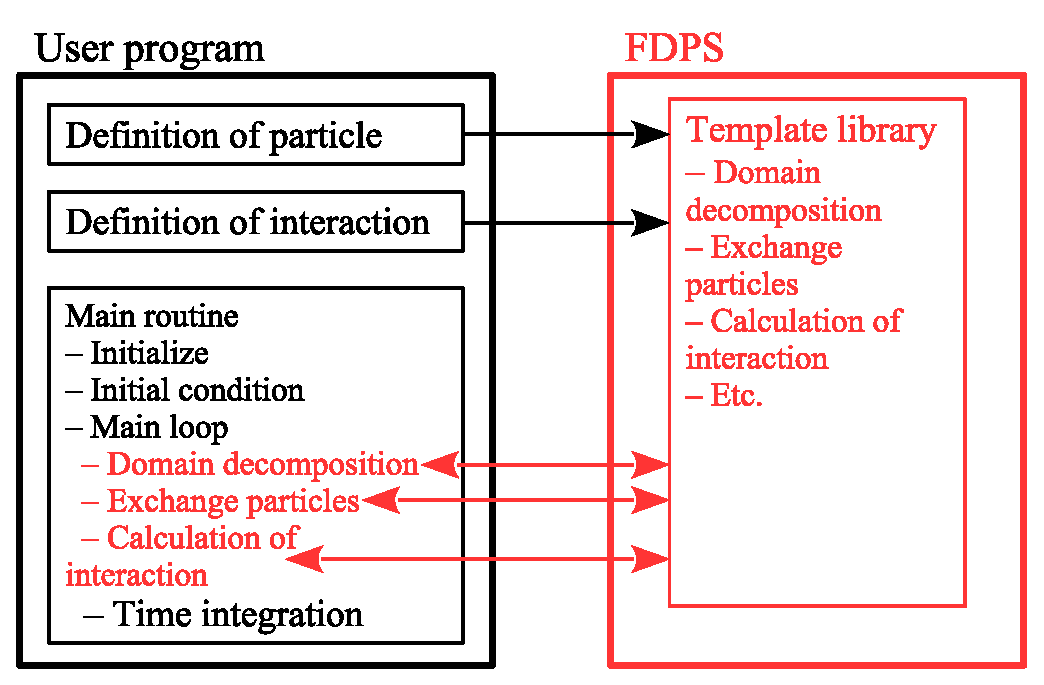
\includegraphics[width=8cm]{fig/concept.eps}
  \end{center}
  \caption{The basic concept of FDPS. The user program gives the
    definitions of particle and interaction to FDPS, and calls FDPS
    APIs.}
  \label{fig:concept}
\end{figure}

A user of FDPS can develop the simulation code in the following three
steps:
\begin{enumerate}
\item Define the data structure for $\myvec{u}_i$, as a class in C++
  language.
\item Define the function $\myvec{f}$. It should be a function object
  in C++ language\footnote{A function pointer of C language can be
    operable.}, which receives arrays of $i$-particles and
  $j$-particles, and calculates and accumulates $\myvec{f}$ on
  $i$-particles.
\item Write the user program using the data class and functions
  provided by FDPS. Currently, the user program should also be written
  in C++.
\end{enumerate}

Figure~\ref{fig:concept} illustrates how the user-defined code and
FDPS functions interact. The user program gives the definition of
particle and particle-particle interaction to FDPS at the compile
time. When executed, the user program first does the initialization
(the setup of MPI communication is done through a single call to an
FDPS initialization function), and the setup of the initial
condition. Then, the main integration loop is executed. In the main
loop, first the domain decomposition and exchange of particles are
performed, and then the calculation of interactions is
performed. These are all done through library calls to FDPS
functions. Finally, the time integration of particles using the
calculated interaction is performed.

In the above description, the interaction calculation is done once per
one iteration of the main loop. It is possible to use integration
schemes which requires multiple evaluations of interaction within a
single timestep, such as Runge-Kutta schemes. One can just call
interaction calculation API of FDPS, with $\myvec{u}_i$ containing
necessary intermediate values.

FDPS takes care of parallelization using MPI, and it can also use
OpenMP parallelization for internal operations and also for
interaction calculation. Thus, an FDPS user does not have to worry
about these issues. The efficient use of the cache memory and the SIMD
execution unit is not directly taken care by the FDPS libraries, but
handled through the interface to the user-defined interaction
calculation function. The interface is defined so that the interaction
calculation is done for multiple $j$-particles and multiple
$i$-particles. Thus, it performs a large amount of calculation, on a
small amount of data, since the calculation cost is the product of the
numbers of $i$- and $j$-particles, and data amount is sum of them.  In
order to make efficient use of the SIMD execution unit, the innermost
loop should be written in such a way that can be recognized as the
candidate of vectorization by the compiler used. The interface is
defined as taking AoS (array of structures) arguments.  Some compilers
for some architecture might not be able to generate the code to
utilize the SIMD unit for AoS data. In such a case, the user should
write the interaction function in which the AoS data is converted
internally to SoA (structure of arrays) data, and converted back to
the AoS form after the interaction is actually calculated.

\begin{figure}
  \begin{center}
    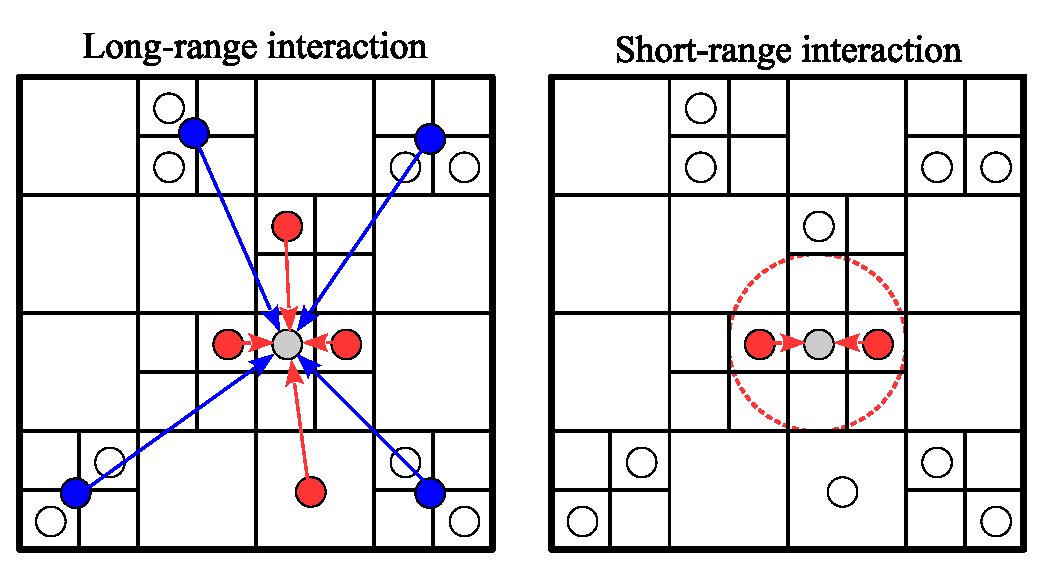
\includegraphics[width=8cm]{fig/force_type.eps}
  \end{center}
  \caption{Long-range interaction (left) and short-range interaction
    (right). Gray, red, and blue points are $i$-particle,
    $j$-particle, and superparticle, respectively.}
  \label{fig:forcetype}
\end{figure}

One might think that the definition of the system given in
equation~(\ref{eq:geq})  implies that  FDPS has to calculate $N^2$
interactions. If that were the case, FDPS would only be useful for
small problems. We implemented $O(N)$ and $O(N\log N)$ calculation
algorithms, for short-range and long-range interactions.

Within FDPS, the difference between long-range and short-range
interactions is slightly different from the physical one of infinite
and finite effective ranges. When we can and want to apply
multipole-like expansion to the contribution from distant particles,
we regard that interaction as long-range. The example of the
long-range interaction is gravity and Coulomb interaction in the open
boundary. When periodic boundary is used, they are usually evaluated
%using $\rm P^3M$ or PME method \cite{hockney1988computer}, in which
using $\mathrm{P^3M}$ or PME method \cite{hockney1988computer}, in
which the long-range part is evaluated using FFT, and only the
interaction with long-range cutoff is evaluated directly.  Even in
this case, we can still apply multipole interaction as used in TreePM
method \cite{1995ApJS...98..355X, 2000ApJS..128..561B,
  2002JApA...23..185B, 2004NewA....9..111D, springel:gadget2,
  2005PASJ...57..849Y, ishiyama:greem, ishiyama:gordonbell}, and in
this case the interaction is treated as long-range in FDPS.

For long-range interactions, FDPS uses standard Barnes-Hut tree
algorithm \cite{1986Natur.324..446B, 1990JCoPh..87..161B} parallelized
for distributed-memory machines and optimized for cache memory and
SIMD units \cite{ishiyama:greem, ishiyama:gordonbell}. For short-range
interactions, interaction list, or ``neighbor list'' for a group of
$i$ particles is constructed using a tree-based search, and that list
is used for the actual interaction calculation.
Figure~\ref{fig:forcetype} illustrates the long-range and short-range
interactions and how they are calculated in FDPS

For the long-range interaction, a multipole-like interaction is
used. Thus, equation~(\ref{eq:geq}) is modified to 
\begin{align}
  \frac{d\myvec{u}_i}{dt} = \myvec{g}\left( \sum_j^{N_{\mathrm{J},i}}
  \myvec{f}(\myvec{u}_i,\myvec{u}_j) + \sum_{j'}^{N_{\mathrm{S},i}}
  \myvec{f'}(\myvec{u}_i,\myvec{u'}_{j'}), \myvec{u}_i
  \right), \label{eq:geqL}
\end{align}
where $N_{\mathrm{J},i}$ and $N_{\mathrm{S},i}$ are, the number of
$j$-particles and superparticles for which we apply multipole-like
expansion, the vector $\myvec{u'}_{j'}$ is the physical quantity
vector of a superparticle, and the function $\myvec{f'}$ indicates the
interaction exerted on particle $i$ by the superparticle $j'$. In
simulations with a large number of particles $N$, $N_{\mathrm{J},i}$
and $N_{\mathrm{S},i}$ are many orders of magnitude smaller than $N$.
The user should also specify how superparticles are constructed from
ordinary particles, and also from superparticles in the lower level of
the tree. For $1/r$ potential, which is the typical usage of the
long-range interaction, FDPS provides the default way of construction
of superparticles up to the quadrupole moment.

In the case of the short-range interaction, the calculation of
contribution of distant particles is suppressed. Thus,
equation~(\ref{eq:geq}) is modified to
\begin{align}
  \frac{d\myvec{u}_i}{dt} = \myvec{g}\left(\sum_j^{N_{\mathrm{J},i}}
  \myvec{f}(\myvec{u}_i,\myvec{u}_j), \myvec{u}_i
  \right), \label{eq:geqS}
\end{align}
As in the case of the long-range force, $N_{\mathrm{J},i}$ is much
smaller than $N$, and usually independent of $N$.



% LocalWords:  FDPS subdomains subdomain MPI parallelization dt discretized API
% LocalWords:  APIs timestep Runge Kutta OpenMP SIMD vectorization AoS SoA PME
% LocalWords:  multipole FFT TreePM parallelized superparticles superparticle
% LocalWords:  quadrupole


\subsection{A working example --- gravitational {\secit N}-body problem}
\label{sec:samplecode}

In this section, we present the complete working example of a
simulation code written using FDPS, to illustrate how a user actually
uses FDPS. As the target problem, we use the gravitational $N$-body
problem with an open boundary.  Within the terminology of FDPS, the
interaction between particles in the gravitational $N$-body problem is
of the ``long-range'' type. Therefore, we need to specify the function
to calculate interactions for both the ordinary particles and
superparticles. For the sake of brevity, we use the center-of-mass
approximation for superparticles, which means we can actually use the
same function for both types of particles.

The physical quantity vector $\myvec{u}_i$ and interaction functions
$\myvec{f}$, $\myvec{f'}$, and $\myvec{g}$ for the gravitational
$N$-body problem is now given by:
\begin{align}
  \myvec{u}_i &= (\myvec{r}_i,
  \myvec{v}_i,m_i) \label{eq:PhysicalVectorNbody} \\
%%  
  \myvec{f} (\myvec{u}_i, \myvec{u}_j) &= \frac{Gm_j \left(
    \myvec{r}_j - \myvec{r}_i \right)}{ \left( |\myvec{r}_j -
    \myvec{r}_i|^2 + \epsilon_i^2
    \right)^{3/2}} \label{eq:ParticleParticleNbody} \\
%%
  \myvec{f'} (\myvec{u}_i, \myvec{u'}_j) &= \frac{Gm_j' \left(
    \myvec{r}_j - \myvec{r'}_i \right)}{ \left( |\myvec{r}_j -
    \myvec{r'}_i|^2 + \epsilon_i^2
    \right)^{3/2}} \label{eq:ParticleSuperparticleNbody} \\
%%
  \myvec{g}(\myvec{F},\myvec{u}_i)  &= (\myvec{v}_i,\myvec{F},0),
\label{eq:ConversionNbody}
\end{align}
where $m_i$, $\myvec{r}_i$, $\myvec{v}_i$, and $\epsilon_i$ are, the
mass, position, velocity, and gravitational softening of particle $i$,
$m_j'$ and $\myvec{r'}_j$ are, the mass and position of a
superparticle $j$, and $G$ is the gravitational constant.  Note that
the shapes of the functions $\myvec{f}$ and $\myvec{f'}$ are the same.

Listing~\ref{code:samplecode} shows the complete code which can be
actually compiled and run, not only on a single-core machine but also
massively-parallel, distributed-memory machines such as the full-node
configuration of the K computer. The total number of lines is only
117.


\begin{lstlisting}[label=code:samplecode,numbers=left,numbersep=5pt,frame=single,basicstyle=\ttfamily,caption=A sample code of $N$-body simulation]
#include <particle_simulator.hpp>
using namespace PS;

class Nbody{
public:
    F64    mass, eps;
    F64vec pos, vel, acc;
    F64vec getPos() const {return pos;}
    F64 getCharge() const {return mass;}
    void copyFromFP(const Nbody &in){ 
        mass = in.mass;
        pos  = in.pos;
        eps  = in.eps;
    }
    void copyFromForce(const Nbody &out) {
        acc = out.acc;
    }    
    void clear() {
        acc = 0.0;
    }
    void readAscii(FILE *fp) {
        fscanf(fp,
               "%lf%lf%lf%lf%lf%lf%lf%lf",
               &mass, &eps,
               &pos.x, &pos.y, &pos.z,
               &vel.x, &vel.y, &vel.z);
    }
    void predict(F64 dt) {
        vel += (0.5 * dt) * acc;
        pos += dt * vel;
    }
    void correct(F64 dt) {
        vel += (0.5 * dt) * acc;
    }
};

template <class TPJ>
struct CalcGrav{
    void operator () (const Nbody * ip,
                      const S32 ni,
                      const TPJ * jp,
                      const S32 nj,
                      Nbody * force) {
        for(S32 i=0; i<ni; i++){
            F64vec xi  = ip[i].pos;
            F64    ep2 = ip[i].eps
                * ip[i].eps;
            F64vec ai = 0.0;
            for(S32 j=0; j<nj;j++){
                F64vec xj = jp[j].pos;
                F64vec dr = xi - xj;
                F64 mj  = jp[j].mass;
                F64 dr2 = dr * dr + ep2;
                F64 dri = 1.0 / sqrt(dr2);                
                ai -= (dri * dri * dri
                       * mj) * dr;
            }
            force[i].acc += ai;
        }
    }
};

template<class Tpsys>
void predict(Tpsys &p,
             const F64 dt) {
    S32 n = p.getNumberOfParticleLocal();
    for(S32 i = 0; i < n; i++)
        p[i].predict(dt);
}

template<class Tpsys>
void correct(Tpsys &p,
             const F64 dt) {
    S32 n = p.getNumberOfParticleLocal();
    for(S32 i = 0; i < n; i++)
        p[i].correct(dt);
}

template <class TDI, class TPS, class TTFF>
void calcGravAllAndWriteBack(TDI &dinfo,
                             TPS &ptcl,
                             TTFF &tree) {
    dinfo.decomposeDomainAll(ptcl);
    ptcl.exchangeParticle(dinfo);    
    tree.calcForceAllAndWriteBack
        (CalcGrav<Nbody>(),
         CalcGrav<SPJMonopole>(),
         ptcl, dinfo);    
}

int main(int argc, char *argv[]) {
    F32 time  = 0.0;
    const F32 tend  = 10.0;
    const F32 dtime = 1.0 / 128.0;
    PS::Initialize(argc, argv);
    PS::DomainInfo dinfo;
    dinfo.initialize();
    PS::ParticleSystem<Nbody> ptcl;
    ptcl.initialize();
    PS::TreeForForceLong<Nbody, Nbody,
        Nbody>::Monopole grav;
    grav.initialize(0);
    ptcl.readParticleAscii(argv[1]);
    calcGravAllAndWriteBack(dinfo,
                            ptcl,
                            grav);
    while(time < tend) {
        predict(ptcl, dtime);        
        calcGravAllAndWriteBack(dinfo,
                                ptcl,
                                grav);
        correct(ptcl, dtime);        
        time += dtime;
    }
    PS::Finalize();
    return 0;
}
\end{lstlisting}


Now let us explain how this sample code works. This code consists of
four parts: The declaration to use FDPS (lines 1 and 2), the
definition of the particle (the vector $\myvec{u}_i$) (lines 4 to 35),
the definition of the gravitational force (the functions $\myvec{f}$
and $\myvec{f'}$) (lines 37 to 61), and the actual user program,
comprising a user-defined main routine and user-defined functions from
which library functions of FDPS are called (lines 63 to line 117). In
the following, we explain them step by step.

In order to declare to use FDPS, the only thing the user program need
to do is to include the header file ``particle\_simulator.hpp''. This
file and other source library files of FDPS should be in the include
path of the compiler. Everything in the standard FDPS library is
provided as the header source library, since they are implemented as
template libraries which need to receive particle class and
interaction functions. Everything in FDPS is provided in the namespace
``PS''. Therefore in this sample program, we declare it as the default
namespace to simplify the code. (For simplicity's sake, we do not omit
the namespace ``PS'' of FDPS functions and class templates in the main
routine.)

Before going to the 2nd parts, let us list the data types and classes
defined in FDPS. \texttt{F32/F64} are data types of 32-bit and 64-bit
floating points. \texttt{S32} is a data type of 32-bit signed integer.
\texttt{F64vec} is a class of a vector consisting of three 64-bit
floating points. This class provides several operators, such as the
addition, subtraction and the inner product indicated by ``$*$''.
Users need not use these data types in their own program, but some of
the functions which users should define should return the values in
these data types.

In the 2nd part, we define the particle, i.e. the vector
$\myvec{u}_i$, as a class \texttt{Nbody}. This class has member
variables: \texttt{mass} ($m_i$), \texttt{eps}
($\epsilon_i$), \texttt{pos} ($\myvec{r}_i$), \texttt{vel}
($\myvec{v}_i$), and \texttt{acc} ($d\myvec{v}_i/dt$). Although the
member variable \texttt{acc} does not appear in
equation~(\ref{eq:PhysicalVectorNbody}) -- (\ref{eq:ConversionNbody}),
we need this variable to store the result of the gravitational force
calculation. A particle class for FDPS must provide public member
functions \texttt{getPos}, \texttt{getCharge}, \texttt{copyFromFP},
\texttt{copyFromForce}, \texttt{clear},
and \texttt{readAscii}, in these names, so that the internal functions
of FDPS can access the data within the particle class.  For the name
of the particle class itself and the names of the member variables, a
user can use whatever names allowed by the C++ syntax.  The member
functions \texttt{predict} and \texttt{correct} are used in the
user-defined part of the code to integrate the orbits of particles.
Note that since the interaction used here is of $1/r$ type, the
definition and construction method of the superparticle are given as
the default in FDPS and not shown here.

In the 3rd part, the interaction functions $\myvec{f}$ and
$\myvec{f'}$ are defined. Since the shapes of the functions
$\myvec{f}$ and $\myvec{f'}$ are the same, we give one as a template
function.  The interaction function used in FDPS should have the
following five arguments. The first argument \texttt{ip} is the
pointer to the array of variables of particle
class \texttt{Nbody}. This argument specifies $i$-particles which
receive the interaction. The second argument \texttt{ni} is the number
of $i$-particles. The third argument \texttt{jp} is the pointer to the
array of variable of a template data type \texttt{TPJ}. This argument
specifies $j$-particles or superparticles which exert the
interaction. The fourth argument \texttt{nj} is the number of
$j$-particles or super-particles. The fifth argument \texttt{force} is
the pointer to the array of a variable of a user-defined class to
which the calculated interaction on an $i$-particle can be stored. In
this example, we used the particle class itself, but this can be
another class or a simple array.

%
The interaction function should be defined as a function object, so
that it can be passed to other functions as argument. Thus, it is
declared as a \texttt{struct}, with the only member
function \texttt{operator ()}.  In this example, the interaction is
calculated through a simple double loop. In order to make full
advantage of the SIMD unit in modern processors,
architecture-dependent tuning may be necessary, but only to this
single function.

In the 4th part, we give the main routine and functions called from
the main routine. In the following, we describe the main routine in
detail, and briefly discuss other functions. The main routine consists
of the following seven steps:
\begin{enumerate}
\item Set simulation time and timestep (lines 92 to 94). \label{proc:literal}
\item Initialize FDPS (line 95). \label{proc:init}
\item Create and initialize objects of FDPS classes (lines 96 to 102). \label{proc:construct}
\item Read in particle data from a file (line 103). \label{proc:input}
\item Calculate the gravitational forces of all the particles at the
  initial time (lines 104 to 106). \label{proc:calcinteraction}
\item Integrate the orbits of all the particles with Leap-Frog method
  (lines 107 to 114). \label{proc:integration}
\item Finish the use of  FDPS (line 115). \label{proc:fin}
\end{enumerate}

In the following, we describe  steps~\ref{proc:init},
\ref{proc:construct}, \ref{proc:input}, \ref{proc:calcinteraction},
and \ref{proc:fin}, and skip steps~\ref{proc:literal}
and \ref{proc:integration}.  In step~\ref{proc:literal}, we do not
call FDPS libraries.  Although we call FDPS libraries in
step~\ref{proc:integration}, the usage is the same as in
step~\ref{proc:calcinteraction}.

In step~\ref{proc:init}, the FDPS function \texttt{Initialize} is
called. In this function, MPI and OpenMP libraries are initialized. If
neither of them are used, this function does nothing.  All functions
of FDPS must be called between this function and the
function \texttt{Finalize}.

In step~\ref{proc:construct}, we create and initialize three objects
of the FDPS classes:
\begin{itemize}
\item \texttt{dinfo}: An object of class \texttt{DomainInfo}. It is
  used for domain decomposition.
\item \texttt{ptcl}: An object of class template \texttt{ParticleSystem}.
It takes the user-defined particle class (in this
example, \texttt{Nbody}) as the template argument. From the user
program, this object looks as an array of $i$-particles.
\item \texttt{grav}: An object of a data type \texttt{Monopole} defined in
a class template \texttt{TreeForForceLong}. This object is used for
the calculation of long-range interaction using the tree algorithm.
It receives three user-defined classes template arguments: the class
to store the calculated interaction, the class for $i$-particles and
the class for $j$-particles. In this example, all three are the same
as the original class of particles.  It is possible to define classes
with minimal data for these purposes and use them here, in order to
optimize the cache usage. The data type \texttt{Monopole} indicates
that the center-of-mass approximation is used for superparticles.
\end{itemize}

In step~\ref{proc:input}, the data of particles are read from a file
into the object \texttt{ptcl}, using the FDPS
function \texttt{readParticleAscii}. In the function, a member
function of class \texttt{Nbody}, \texttt{readAscii}, is called.

In step~\ref{proc:calcinteraction}, the forces on all particles are
calculated through the function \texttt{calcGravAllAndWriteBack}, which
is defined in lines 79 to 89. In this function,
steps~\ref{proc:decompose}, \ref{proc:exchange}, and
\ref{proc:interaction} in section~\ref{sec:view} are performed. In
other words, all of the actual work of FDPS libraries to calculate
interaction between particles takes place here. For
step~\ref{proc:decompose}, \texttt{decomposeDomainAll}, a member function
of class \texttt{DomainInfo} is called. This function takes the object
\texttt{ptcl} as an argument to use the positions of particles to
determine the domain decomposition.  Step~\ref{proc:exchange} was
performed in \texttt{exchangeParticle}, a member function of
class \texttt{ParticleSystem}. This function takes the
object \texttt{dinfo} as an argument and redistributes particles among
MPI processes.  Step~\ref{proc:interaction} was performed
in \texttt{calcForceAllAndWriteBack}, a member function of
class \texttt{TreeForForceLong}. This function takes the user-defined
function object \texttt{CalcGrav} as the first and second arguments,
and calculates particle-particle and particle-superparticle
interactions using them.

In step~\ref{proc:fin}, the FDPS function \texttt{Finalize} is
called. It calls the \texttt{MPI\_finalize} function.

In this section, we have described in detail how a user program
written using FDPS looks like. As we stated earlier, this program can
be compiled with or without parallelization using MPI and/or OpenMP,
without any change in the user program. The executable parallelized
with MPI is generated by using an appropriate compiler with MPI
support and a compile-time flag.  Thus, a user need not worry about
complicated bookkeeping necessary for parallelization using MPI.
%
In the next section, we describe how FDPS provides a generic
framework which takes care of parallelization
and bookkeeping for particle-based simulations. 

% LocalWords:  monopole superparticle FDPS hpp namespace nd th vec Nbody eps dt
% LocalWords:  pos vel acc getPos getCharge copyFromFP copyFromForce readAscii
% LocalWords:  ip const ni jp TPJ nj MPI OpenMP DomainInfo dinfo subdomains
% LocalWords:  subdomain ParticleSystem ptcl TreeForForceLong readParticleAscii
% LocalWords:  calcGravAllAndWriteBack decomposeDomainAll exchangeParticle SIMD
% LocalWords:  calcForceAllAndWriteBack CalcGrav superparticles struct grav
% LocalWords:  parallelization parallelized timestep


\section{Implementation}
\label{sec:implementation}

In this section, we describe how the operations discussed in the
previous section are implemented in FDPS. In
section~\ref{sec:decomposition} we describe the domain decomposition
and particle exchange, and in section~\ref{sec:calculation}, the
calculation of interactions.

\subsection{Domain decomposition and particle exchange}
\label{sec:decomposition}

In this section, we describe how the domain decomposition and the
exchange of particles are implemented in FDPS. We used the
multisection method
\citep{2004PASJ...56..521M} with the so-called sampling
method \citep{Blackston:1997:HPE:509593.509597}. The multisection
method is a generalization of ORB (Orthogonal Recursive Bisection). In
ORB, as its name suggests, bisection is applied to each coordinate
axis recursively. In multisection method, division in one coordinate
is not to two domains but to an arbitrary number of domains. Since one
dimension can be divided to more than two sections, it is not
necessary to apply divisions many times. So we apply divisions only
once to each coordinate axis. A practical advantage of this method is
that the number of processors is not limited to powers of two.

Figure~\ref{fig:decomposition} illustrates an example of the
multisection method with $(n_x, n_y, n_z)=(7,6,1)$. We can see that
the size and shape of subdomains show large variation. By allowing
this variation, FDPS achieves quite good load balance and high
scalability. Note that $n=n_x n_y n_z$ is the number of MPI
processes. By default, values of $n_x$, $n_y$, and $n_z$ are chosen so
that they are integers close to $n^{1/3}$. For figure
~\ref{fig:decomposition}, we force the numbers used to make a
two-dimensional decomposition.

\begin{figure}
  \begin{center}
    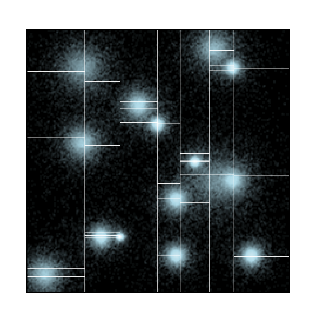
\includegraphics[width=8cm]{figure/pm3d.eps}
  \end{center}
  \caption{Example of the domain decomposition. The division is $7
    \times 6$ in 2-dimension.}
  \label{fig:decomposition}
\end{figure}


In the sampling method, first each process performs random sampling of
particles under it, and sends them to the process with rank 0
(``root'' process hereafter). Then the root process calculates the
division so that sample particles are equally divided over all
processes, and broadcasts the geometry of domains to all other
processes. In order to achieve good load balance, sampling frequency
should be changed according to the calculation cost per particle
\citep{2009PASJ...61.1319I}.

The sampling method works fine, if the number of particles per process
is significantly larger than the number of process. This is, however,
not the case for runs with a large number of nodes.  When the number
of particles per process is not much larger than the number of
processes, the total number of sample particles which the root process
needs to handle exceeds the number of particles per process itself,
and thus calculation time of domain decomposition in the root process
becomes visible.

%For example, K computer has more than 80,000 nodes, and in this paper
%we report the result of runs with all nodes. Even with Even with the
%number of particles per process same as the number of nodes, the
%total number of particles becomes 6.4 billion, and we do want to run
%simulations with smaller number of particles.

In order to reduce the calculation time, we also parallelized the
domain decomposition, currently in the direction of $x$ axis only. The
basic idea is that each node sends the sample particles not to the
root process of the all MPI processes but to the processes with index
$(i,0,0)$. Then processes $(i,0,0)$ sort the sample particles and
exchange the number of sample particles they received. Using these two
pieces of information, each of $(i,0,0)$ processes can determine all
domain boundaries inside its current domain in the $x$ direction. Thus,
they can determine which sample particles should be sent to
where. After the exchange of sample particles, each of $(i,0,0)$
processes can determine the decompositions in $y$ and $z$ directions.

A naive implementation of the above algorithm requires ``global''
sorting of sample particles over all of $(i,0,0)$ processes. In order
to simplify this part, before each process sends the sample particles
to  $(i,0,0)$ processes, they exchange their samples with other
processes with the same location in $y$ and $z$ process coordinates, so
that they have sample particles in the current domain decomposition in
the x direction. As a result, particles sent to $(i,0,0)$ processes
are already sorted at the level of domains decomposition in $x$
direction, and we need only the  sorting within each of $(i,0,0)$
processes to obtain the globally sorted particles.

Thus, our implementation of parallelized domain decomposition
is as follows:

\begin{enumerate}
\item
Each process samples particles randomly from its own particles. In
order to achieve an optimal load balance, the sampling rate of
particles is changed so that it is proportional to the CPU time per
particle spent on that process \citep{2009PASJ...61.1319I}. FDPS
provides several options including this optimal
balance. \label{prcoc:sampling}

%%
\item
Each process exchanges the sample particles according to the current
domain boundary in the $x$ direction with the process with the same y
and z indices, so that they have sample particles in the current
domain decomposition in the $x$ direction.


\label{proc:commx}

%%
\item
Each process with index $(i,y,z)$ sends the sample particles to the
process with index $(i,0,0)$, in other words, the root processes in
each of $y$-$z$ planes collects subsamples.

\label{proc:gatherx}

%%
\item
Each root process sorts the sample particles in the $x$ direction. Now,
the sample particles are sorted globally in the $x$ direction.

%%
\item
Each root process sends the number of the sample particles to the
other root processes and determines the global rank of the sample
particles.

%%
\item
Determine the $x$ coordinate of new domains by dividing all sample
particles into $n_x$ subsets with equal number of sample particles.
\label{proc:determinex}

%%
\item
Each root process exchanges sample particles with other root
processes, so that they have the sample particles in new domain in the
$x$ direction.

%\ref{proc:determinex}.

%of which $x$ coordinate is in the range of
%the $x$ coordinate of new subdomain determined in
%step

%%
\item
Each root process determines the $y$ and $z$ coordinates of new domains.
\label{proc:detyz}

%%
\item
Each root process broadcasts the geometries of new domains to all
other processes.
\label{proc:broadcasting}

\end{enumerate}

It is also possible to parallelize  the determination of  subdomains in
step \ref{proc:detyz}, but even for the full-node runs on K computer
we found the current parallelization is sufficient.

For particle exchange and also for interaction information exchange,
we use {\tt MPI\_Alltoall} to exchange the length of the data and {\tt
MPI\_Isend} and {\tt MPI\_Irecv} to actually exchange the data. At
least on K computer, we found that the performance of vendor-provided
{\tt MPI\_Alltoall} is not optimal for short messages. We implemented
a hand-crafted version in which the messages sent to the same relay
points are combined in order to reduce the total number of messages.


After the domain decomposition is done and the result is broadcasted
to all processes, they exchange particles so that each of them has
particles in its domain. Since each process has the complete
information of the domain decomposition, this part is pretty
straightforward to implement. Each process looks at each of its
particles, and determines if that particle is still in its domain.  If
not, the process determines to which process that particle should be
sent. After the destinations of all particles are determined, each
process sends them out, using {\tt MPI\_Isend} and {\tt MPI\_Irecv}
functions.


% LocalWords:  FDPS subdomain MPI multi subdomains DomainInfo ParticleSystem
% LocalWords:  decomposeDomainAll exchangeParticle substeps scalability
% LocalWords:  broadcasted Alltoallv


\subsection{Interaction calculation}
\label{sec:calculation}

In this section, we describe the implementation of the calculation of
interactions in FDPS. Conceptually, it consists of the following two
steps. In the first step, each process determines, for each of other
processes, which of its particles and superparticles are required by
that process for interaction calculation, and sends them to it. In the
second step, each process calculates the interactions onto
$i$-particles by calling user-defined function objects.

\if 0
\begin{enumerate}
\item Each process determines, for each of other processes, which of
  its particles and   superparticles are required by that process for
  interaction calculation,   and sends them to it.

%%
\item Each process calculates the interactions onto  $i$-particles by
  calling user-defined function objects.
\end{enumerate}
\fi

\begin{figure}
  \begin{center}
    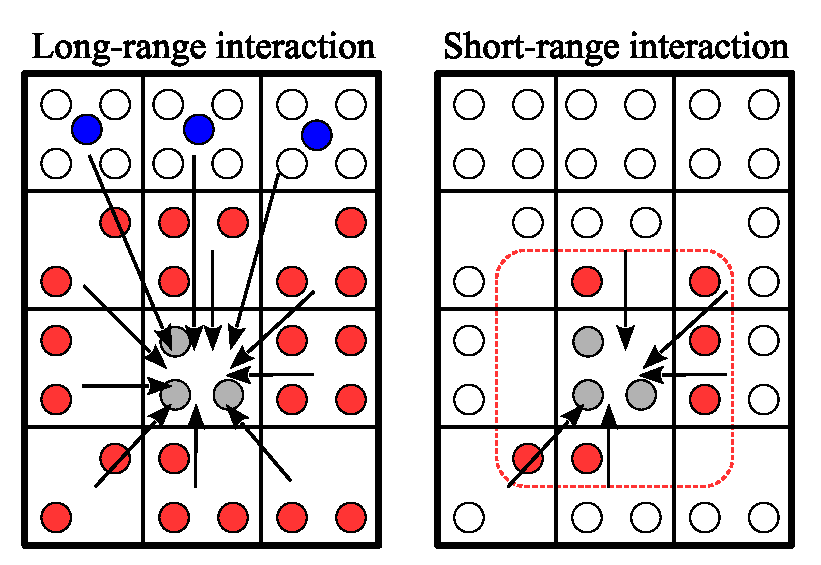
\includegraphics[width=8cm]{fig/exchangeLET.eps}
  \end{center}
  \caption{Illustration of communication among processes during the
    interaction calculation.}
  \label{fig:exchangeLET}
\end{figure}

For both steps, the octree structure is used, both for long- and
short-range interactions.
%%In step 1, 
In the first step, each process constructs the tree structure for its
local particles, and uses it to determine what data should be sent to
other processes. For the long-range interactions, this part is done
through the usual tree traversal \cite{1986Natur.324..446B,
  1990JCoPh..87..161B}. For the short-range interactions, tree
traversal is also used. A cube in a tree need to be subdivided if it
is within the cutoff length from anywhere in the domain of the process
to which the data will be sent.  The current implementation of FDPS
can handle four different types of the cutoff length for the
``short-range'' interaction: fixed, $j$-dependent, $i$-dependent and
symmetric.  For $i$-dependent and symmetric cutoffs, FDPS does the
tree traversal twice.  Figure~\ref{fig:exchangeLET} illustrates what
data are sent, for both long- and short-range interactions.

After a process receives all data it requires, it reconstructs the
tree structure which contains all information necessary to calculate
interactions on its particles.

The interaction calculation is performed using this new tree. The
procedure is the same as described in detail in the literature
\cite{1990JCoPh..87..161B, 1991PASJ...43..859M}, except for the
following two differences.  First, this part is fully multithreaded
using OpenMP, to achieve very good parallel performance. Second, for
the interaction calculation the user-provided functions are used, to
achieve the flexibility and high performance at the same time.

% LocalWords:  FDPS TreeForForceLong TreeForForceShort calcForceAllAndWriteBack
% LocalWords:  subdomains substeps octree multipole superparticles nd OpenMP
% LocalWords:  substep multithreading multithreaded


\section{Performance}
\label{sec:performance}

In this section, we report the performance of two astrophysical
applications of FDPS: a gravitational $N$-body simulation code in
section~\ref{sec:nbody} and an SPH simulation code with self-gravity
in \ref{sec:sph}.

\subsection{{\secit N}-body simulation}
\label{sec:nbody}

In this section, we discuss the performance and scalability of a
gravitational $N$-body simulation code implemented using FDPS. The
code is essentially the same as the sample code described in
section~\ref{sec:samplecode}, except for the following two differences
in the user code for the calculation of the interaction. First, here,
we used the expansion up to quadrupole moment, instead of
monopole-only one used in the sample code, to improve the
accuracy. Second, we used highly-optimized kernel developed using SIMD
builtin functions, instead of the simple one in the sample code.

We use the Plummer model \cite{1911MNRAS..71..460P} to realize
particle distribution at the initial time. We adopt $\theta=0.4$ for
the opening angle for the tree algorithm. In this paper, we present
the weak-scaling performance of the code with FDPS. Therefore we fixed
the number of particles per core to $250$ thousands.

\begin{figure}
  \begin{center}
%      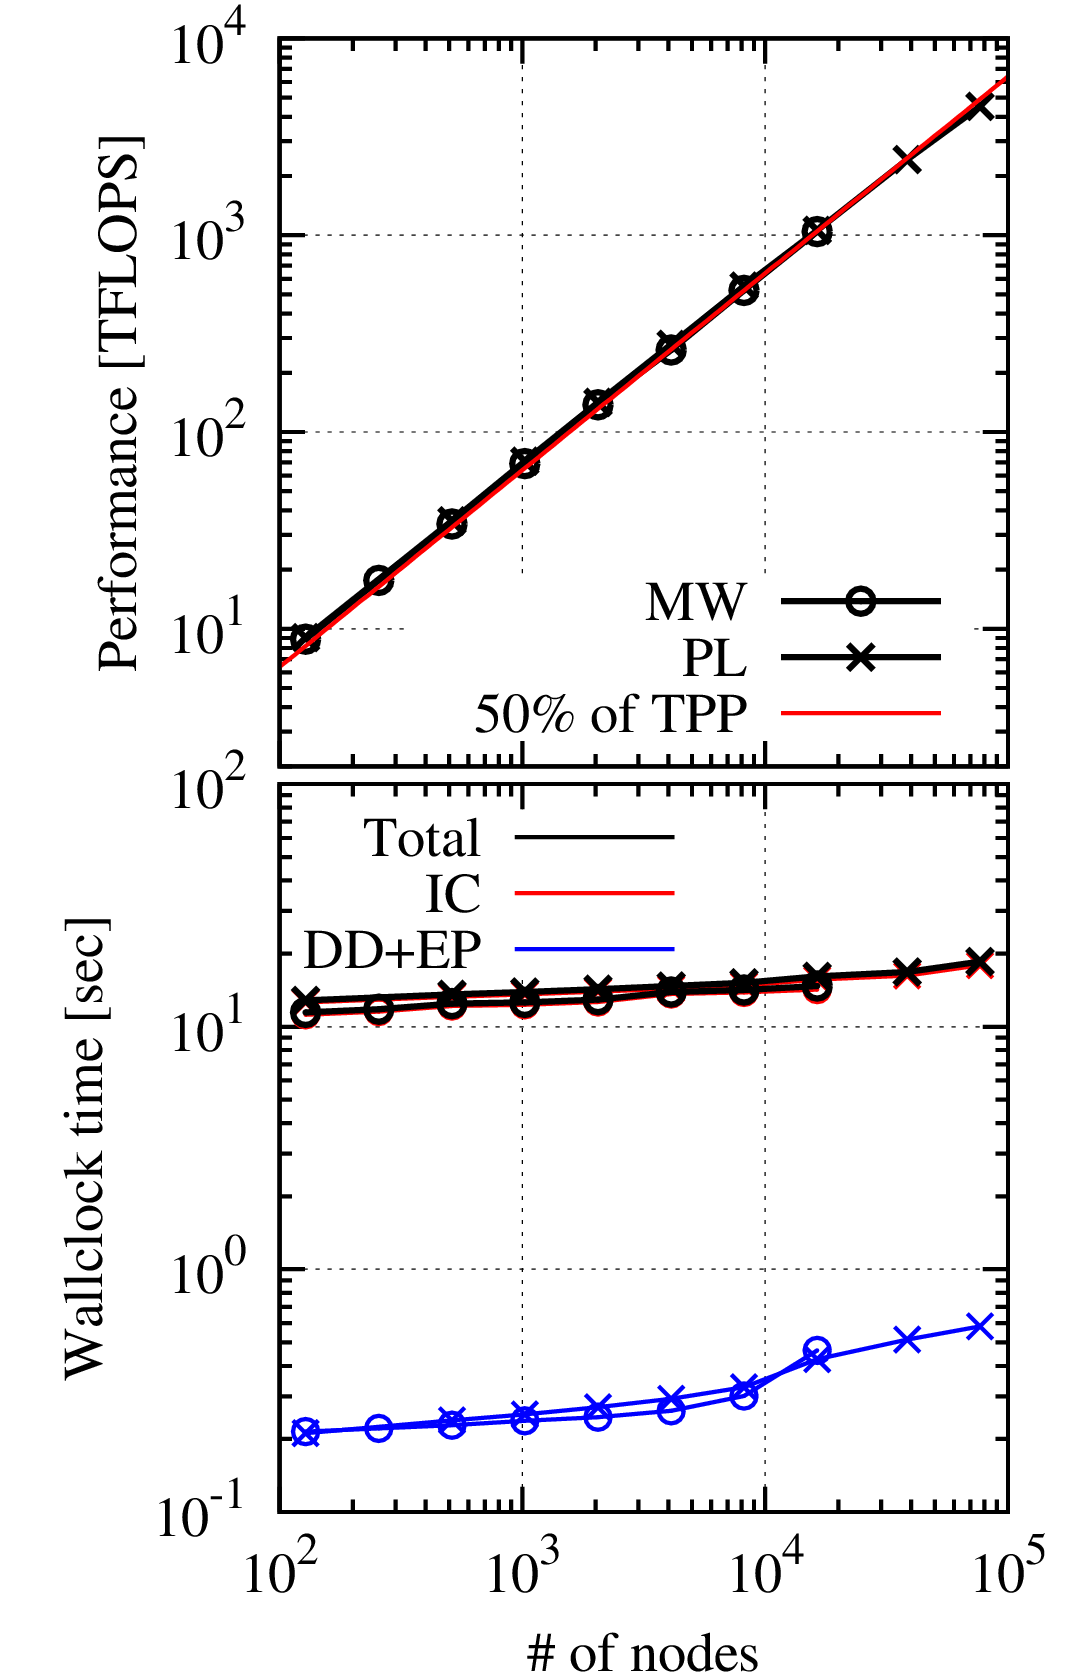
\includegraphics[width=8cm,bb=0 0 540 840]{../sandbox/tanikawa_box/figure/ws_sc15/bench.png}
      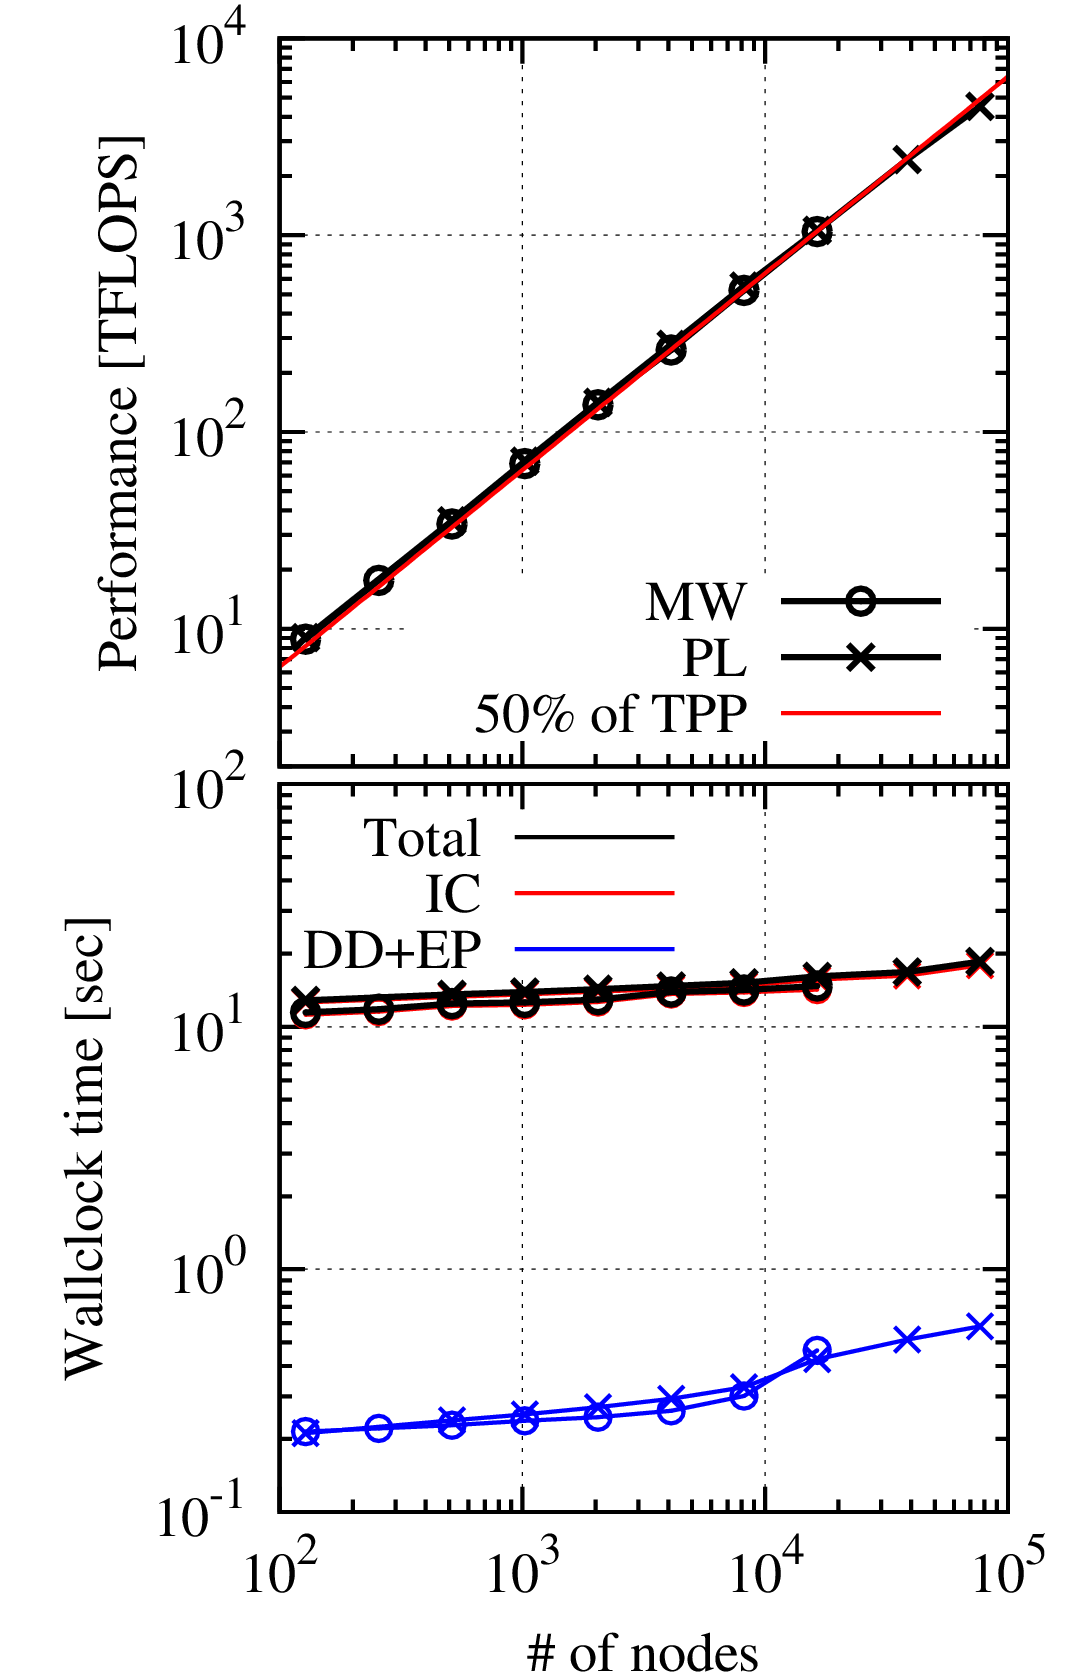
\includegraphics[width=7.5cm,bb=0 0 540 840]{../sandbox/tanikawa_box/figure/ws_sc15/bench.png}
  \end{center}
  \caption{Performance measured in the speed of the floating-point
    operation (top) and wallclock time per one timestep (bottom)
    plotted as functions of the number of cores. Filled and open
    points indicate the performance on K computer and Cray XC30,
    respectively. Square and circle points show the performance of our
    SPH simulation code and $N$-body simulation code, respectively.}
  \label{fig:benchdisk}
\end{figure}

We run our $N$-body simulation code on two platforms: K computer at
RIKEN Advanced Institute for Computational Science, and Cray XC30
(with Haswell processors) at National Astronomical Observatory of
Japan. The maximum numbers of cores we used are $612352$ cores
($76544$ nodes) on K computer, and $2064$ cores ($86$ nodes) on Cray
XC30. The run using $612352$ cores on K computer is almost a
full-system one, where the full-system run operates $663552$ cores.
Precision of floating point for interaction calculations is double on
K computer, and single on Cray XC30. The single floating point
precision is sufficient for the scientific calculation on this
field. Since the performance of the single floating point precision is
the same as that of the double one on K computer, we adopt the double
one for the calculation on K computer.

Filled and open circles in Figure~\ref{fig:benchdisk} show the
measured performance of our $N$-body simulation code. We can see the
measured efficiency and scalability are both very good on both
platforms. On K computer, efficiency is very close to 50\% for the
entire range of nodes. Wallclock time shows slight increase for larger
number of nodes, but this is due to the increase of the calculation
cost and not due to the degradation of the efficiency. The performance
on Cray XC30 is about $4$ times higher than that on K computer, since
the peak performance per core in single floating point precision on
Cary XC30 is about $5$ times higher than that in double floating point
precision on K computer

We compare the performance of our $N$-body simulation code with that
of GreeM code \cite{ishiyama:greem, ishiyama:gordonbell}. GreeM code
treats $N$-body simulation with TreePM algorithm, and was awarded the
2012 ACM Gordon Bell Prize. The wallclock times of GreeM and our codes
are $2.80 \times 10^{-11}$ and $1.16 \times 10^{-10}$
sec/step/particle. Our code using FDPS seems to be $4$ times slower
than GreeM. However, this is due to the difference of the algorithms
used. Since TreePM algorithm calculates forces from distant particles
by Fast Fourier Transform, the number of particle-particle
interactions in TreePM algorithm is much smaller than that in the tree
algorithm. Therefore, comparison of the wallclock time per interaction
is more fair. The wallclock time is $1.14 \times 10^{-14}$ (GreeM) and
$1.71 \times 10^{-14}$ (ours) sec/step/interaction. The performance is
comparable, even though the number of particles per node is smaller by
a factor of $6$. The performance of GreeM was measured for
$1.6$ million particles per core, while we used $250$ thousand
particles per core.

%%%% about comparison ...

%% ours     1.16 x 10^-10 sec/step/particle
%% ishiyama 2.80 x 10^-11 sec/step/particle

%% ours     1.71 x 10^-14 sec/step/interaction
%% ishiyama 1.14 x 10^-14 sec/step/interaction

%B\'edorf \textit{et al.}\cite{Bedorf:2014:PGT:2683593.2683600}
%reported the wallclock time of 4 seconds for their 27-billion
%particle simulation on the Titan system with 2048 NVIDIA Tesla K20X,
%with the theoretical peak performance of 8PF (single precision, since
%single precision us used for interaction calculation). This
%corresponds to 0.8 billion particles per second per petaflops. Our
%code on K computer requires 15 seconds on 16384 nodes (2PF
%theoretical peak), resulting in 1 billion particles per second per
%petaflops. Therefore, we can conclude that our FDPS code achieved the
%performance slightly better than one of the best codes specialized to
%gravitational $N$-body problem.

% LocalWords:  FDPS superparticle monopole quadrupole SIMD builtin Hernquist IC
% LocalWords:  Frenk NFW EP scalability TPP PFLOPS NVIDIA kpc axisymmetric pc
% LocalWords:  GalacticICS Gyrs timestep edorf et al petaflops Wallclock
% LocalWords:  wallclock


\subsection{SPH simulation}
\label{sec:sph}

In this section, we discuss the performance of an SPH simulation code
with self-gravity implemented using FDPS. The test problem used is the
simulation of Giant Impact (GI). The giant impact
hypothesis \cite{1975Icar...24..504H, 1976LPI.....7..120C} is one of
the most popular scenarios for the formation of the Moon. The
hypothesis is as follows. About 5 billion years ago, a Mars-sized
object (hereafter, the impactor) collided with the proto-Earth
(hereafter, the target). The collision scattered a large amount of
debris, which first formed the debris disk and eventually the
Moon. Many researchers have performed simulations of GI, using the SPH
method.
\cite{1986Icar...66..515B, 2013Icar..222..200C, 2014NatGe...7..564A}.

For the gravity, we used monopole-only kernel with $\theta=0.5$. We
adopt the standard SPH scheme
\cite{1992ARA&A..30..543M, 2009NewAR..53...78R, 2010ARA&A..48..391S}
for the hydro part. Artificial viscosity was used to handle shock waves
\cite{1997JCoPh.136..298M}, and 
the standard Balsara switch was used to reduce the shear viscosity
\cite{1995JCoPh.121..357B}. Assuming that the target and impactor
consist of granite, we adopt the equation of state of
granite \cite{1986Icar...66..515B} for the particles. The initial
conditions, such as the orbital parameters of the two objects, are the
same as those in \cite{1986Icar...66..515B}. In this paper, we report
the weak scaling performance with about 250k particles per node. For
the largest calculation, we used $1.0$ billion particles and $4096$
nodes.

Similarly to our $N$-body simulation code, we run our SPH simulation
code on K computer and Cray XC30. The maximum numbers of cores we used
are $32768$ cores ($4096$ nodes) on K computer, and $2064$ cores ($86$
nodes) on Cray XC30.

For gravity calculations, we used highly-optimized kernel developed
using SIMD builtin functions on both platforms. However, for fluid
calculations, we used the optimized kernel on the K computer, but do
not on Cray XC30.

\begin{figure}
  \begin{center}
%    \includegraphics[width=8cm]{fig/GI.eps}
    \includegraphics[width=7cm]{fig/GI.eps}
  \end{center}
  \caption{Temperature maps of the target and impactor in the run of
  $9.9$ million particles at four different epochs. }
  \label{fig:evolutionGI}
\end{figure}

Figure~\ref{fig:evolutionGI} shows the time evolution of the target
and impactor for a run with 9.9 million particles. We can see that the
shock waves are formed just after the moment of impact in both the
target and impactor (t=2050sec). The shock propagates in the target,
while the impactor is completely disrupted (t=2847sec) and debris is
ejected. Part of the debris falls back to the target, while the rest
will eventually form the disk and the Moon. So far, the resolution
used in the published papers have been much lower. We plan to use this
code to improve the accuracy of the GI simulations.

Filled and open squares in Figure~\ref{fig:benchdisk} show the
measured performance of our SPH simulation code. We can see the
measured efficiency and scalability are both very good on both
platforms, similarly to our $N$-body simulation code in the previous
section. On the K computer, efficiency is very close to 40\% for the
entire range of the number of nodes. The difference of SPH performance
between K computer and Cray XC30 is smaller than that of $N$-body
performance. This is because our SPH simulation code on Cray XC30 does
not efficiently utilize SIMD instructions for fluid
calculations. Although the SIMD instructions are used for gravity
calculations, the calculation cost is dominated by fluid calculations.

The largest number of particles used for GI simulations so far
reported is 100 million \cite{2014LPI....45.2703T}. Unfortunately,
performance numbers are not given. After we replace the interaction
kernels with SIMD-optimized ones for hydrodynamics part, we believe we
can achieve the performance not so much lower than that we achieved
for pure gravity calculation.

% LocalWords:  SPH FDPS impactor proto Balsara rr rrr Grav Wendland SIMD

% LocalWords:  builtin Wallclock timestep wallclock monopole


\section{Conclusion}
\label{sec:conclusion}

We have developed a novel framework for particle-based simulations,
FDPS.  Users of FDPS need not care about complex implementations of
domain decomposition, exchange of particles, communication of data for
the interaction calculation, or optimization for multi-core
processors.  Using FDPS, particle simulation codes which achieve high
performance and high scalability on massively parallel
distributed-memory machines can be easily developed for a variety of
problems.  As we have shown in section~\ref{sec:samplecode}, a
parallel $N$-body simulation code can be written in less than 120
lines.  Example implementations of gravitational $N$-body simulation
and SPH simulation showed excellent scalability and performance. We
hope FDPS will help researchers to concentrate on their research, by
removing the burden of complex code development for parallization and
architecture-dependent tuning.


% LocalWords:  FDPS multi SPH parallization scalability


%FDPS, \textit{FDPS}, \textbf{FDPS}, \texttt{FDPS}
%\section{Section \secit{Section}}
%\subsection{Subsection \subsecit{Subsection}}
%\subsubsection{Subsubsection}
%\paragraph{Paragraph}
%\paragraph*{Paragraph*}
%$c_\mathrm{s}$, $c_{\mathrm{s},i}$

\section{Acknowledgments}

We thank M. Fujii for providing initial conditions of spiral
simulations, T. Ishiyama for providing his Particle Mesh code, and
Y. Maruyama for being the first user of FDPS.  We are grateful to
M. Tsubouchi for her help in managing the FDPS development team. This
research used computational resources of the K computer provided by
the RIKEN Advanced Institute for Computational Science through the
HPCI System Research project (Project ID:ra000008). Numerical
computations were in part carried out on Cray XC30 at Center for
Computational Astrophysics, National Astronomical Observatory of
Japan.

\bibliographystyle{abbrv}
\bibliography{ws_sc15}

\end{document}

% LocalWords:  FDPS Masaki Iwasawa RIKEN Minatojima minami machi Chuo ku Hyogo
% LocalWords:  Ataru Tanikawa Natsuki Hosono Keigo Nitadori Takayuki Muranushi
% LocalWords:  Junichiro Makino parallelization scalability meshfree multi SIMD
% LocalWords:  Github GreeM SPH APIs du dt sc fdps Fujii Ishiyama Maruyama HPCI
% LocalWords:  Tsubouchi ra
